\chapter{Normas de vectores y matrices}
\section{Normas y producto escalar}


Dado un punto $P = (x,y)$ en el plano, podemos calcular su distancia al origen por el teorema de Pitágoras:
$$
z = \sqrt{x^2 + y^2}.
$$

Generalizando esa fórmula a espacios de cualquier dimensión, obtenemos una norma vectorial:
$$
\|v\|_2 = \sqrt{v_1^2 + \dots + v_n^2}.
$$

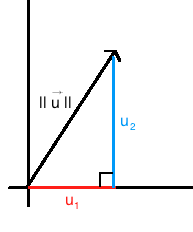
\includegraphics[scale=0.5]{normaVector.png}

Esta norma suele llamarse norma-2 o norma euclídea.

En general, una norma de un $K$-espacio vectorial es una función $\| \cdot \| : V \rightarrow \R_{\ge 0}$ que cumple las siguientes propiedades:
\begin{enumerate}
\item $\|a v\| = |a| \|v\|$, para $a \in \K$ y $v \in V$.
\item Si $\|v\| = 0$, entonces $v = 0$.
\item $\|u + v\| \le \|u\| + \|v\|$, para todo $u, v \in V$
\end{enumerate}

La \'ultima propiedad se denomina desigualdad triangular. Si pensamos a $u$ y $v$ como catetos de un tri\'angulo, $u + v$ es el tercer cateto. Por lo tanto la propiedad nos dice que la longitud de un cateto de un triángulo es siempre menor o igual que la suma de las longitudes de los otros catetos.

Es fácil ver que la norma-2 cumple las primeras dos propiedades.  La demostraci\'on de la tercera propiedad es m\'as dif\'icil y se basa en la siguiente desigualdad clásica.

\begin{prop}[Desigualdad de Cauchy-Schwarz]
Dados $u, v \in \R^n$,
$$
\left(\sum_{i=1}^{n} u_{i}v_{i}\right)^{2}\leq \left(\sum_{i=1}^{n}u_{i}^{2}\right)\left(\sum_{i=1}^{n}v_{i}^{2}\right).
$$
\end{prop}
\begin{proof}
Consideramos el siguiente polinomio de grado 2 en $x$:
$$
p(x) = (u_1 x + v_1)^2 + \dots + (u_n x v_n)^2 = =\left(\sum _{i}u_{i}^{2}\right)x^{2}+2\left(\sum _{i}u_{i}v_{i}\right)x+\sum _{i}v_{i}^{2}.
$$

Como $p$ es una suma de cuadrados, $p(x) \ge 0$ para todo $x \in \R$. Recordemos que las raíces de un polinomio de grado 2 $ax^2 + bx + c$ son $\frac{-b \pm \sqrt{b^2 - 4ac}}{2a}$. Por lo tanto, si un polinomio tiene $0$ o $1$ ra\'iz, debe ser $b^2-4ac \le 0$. En nuestro caso,
$$
4 \left(\sum _{i}u_{i}v_{i}\right)^{2}- 4 \left(\sum _{i}{u_{i}^{2}}\right)\left(\sum _{i}{v_{i}^{2}}\right)\leq 0,
$$
y eliminando el factor 4 y despejando, obtenemos la desigualdad buscada.
\end{proof}

Podemos definir otras normas en un espacio vectorial:

\begin{itemize}
\item Norma-1: $\| v \|_1 = |v_1| + \dots + |v_n|$
\item Norma-infinito: $\| v \|_\infty = \max\{|v_1|, \dots, |v_n|\}$
\item Norma-p: $\| v \|_p = \left(|v_1|^p  + \dots + |v_n|^p \right)^{1/p}$
\end{itemize}

En el siguiente gr\'afico podemos ver la diferencia entre las 3 normas m\'as usuales. En cada gr\'afico est\'an representados todos los puntos con norma igual a 1 bajo la norma respectiva.

\begin{center}

\includegraphics[scale=.35]{140px-Vector_norms.png}
\end{center}

\begin{aplicacion}
Para entender la diferencia entre las distintas normas, analizamos el siguiente ejercicio: Hallar gr\'aficamente el punto del plano de norma igual a 1 que maximiza la funci\'on $f(x,y) = 2y + x$. Para resolverlo, graficamos en el plano todos los puntos para los cuales $f$ tiene un valor fijo. Por ejemplo, los puntos para los cuales $f(x,y) = 3$ se encuentran en una recta que paso por el punto $(3,0)$ y tiene pendiente $-1/2$. Si aumentamos o disminuimos este valor fijo, obtendremos una recta paralela a la anterior desplazada hacia la derecha o izquierda respectivamente.

Por lo tanto, para resolver el problema, desplazamos la recta que trazamos hacia la izquierda hasta que toque a alguno de los puntos de norma 1.
Concluimos que en el caso de la norma-1 este punto es el punto $(1,0)$, para la norma infinito este punto es el punto $(1,1)$ y para la norma 2, este punto es un punto en el arco del primer cuadrante.

En general, al maximizar o minimizar la norma-1 de una función, obtendremos puntos con varias coordenadas nulas, mientras que al minimazar la norma-2 encontraremos puntos con coordenadas no nulas de valor menor que las de la norma-1. Dependiendo la aplicación resultará m\'as \'util una u otra de las normas.
\end{aplicacion}

\subsection{Equivalencia de normas}

Si bien vimos que las normas pueden dar valores distintos, existen relaciones entre las mismas.

\begin{ejercicio}
Probar las siguientes relaciones entre las normas:
\begin{enumerate}
\item $\|x\|_2 \le \|x\|_1 \le \sqrt{n} \|x\|_2$
\item $\|x\|_\infty \le \|x\|_2 \le \sqrt{n} \|x\|_\infty$
\item $\|x\|_\infty \le \|x\|_1 \le n \|x\|_\infty$
\end{enumerate}
\end{ejercicio}

Estas relaciones nos dicen intuitivamente que si un vector tiene norma pequeña bajo una de las normas, tambi\'en lo tendr\'a bajo las otras normas. Para poder precisar este resultado, hacemos la siguiente definici\'on.

\begin{defi}
Decimos que una sucesi\'on de vectores $\{v_n\}_{n \in \N}$ converge bajo una norma $\|\cdot\|$ a un vector $v$ si
$$
\|v_n - v\| \rightarrow 0 \quad \text{ cuando } n \rightarrow \infty.
$$
\end{defi}

\begin{ejercicio}
Dada una sucesi\'on de vectores $\{v_n\}$ que converge a un vector $v$ bajo una de las normas $\|\cdot\|_1$, $\|\cdot\|_2$ o $\|\cdot\|_\infty$, probar que tambi\'en converge para cualquiera de las otras normas.
\end{ejercicio}

Sugerencia: utilizar las relaciones entre normas del ejercicio anterior. Estas relaciones se pueden enunciar en forma general de la siguiente forma. Dadas dos normas $\|\cdot\|_a$ y $\|\cdot\|_b$ en un $\R$-espacio vectorial $V$, existen constantes $c_1$ y $c_2$ tales que $c_1 \|v\|_a \le \|v\|_b \le c_2 \|v\|_b$. Observar que si bien aparecen en las relaciones algunos coeficientes que dependen de $n$, al fijar el espacio vectorial $V$ el valor de $n$ queda fijo y por lo tanto, podemos tomar esos coeficientes como constantes.

\subsection{Distancia entre dos puntos}

A partir de una norma en $V$, podemos definir una distancia en $V$:
$$
d(\ub, \vb) = \|\vb - \ub\|, \text{ para } \ub, \vb \in V.
$$

A partir de ahora trabajamos siempre con la norma-2.

\begin{ejemplo}
La distancia entre dos puntos (o vectores) $P_1 = (x_1, y_1)$ y $P_2 = (x_2, y_2)$ de $V$ queda definida por la fórmula
$$
d(P_1, P_2) = \sqrt{(x_2-x_1)^2 + (y_2 - y_1)^2}
$$
\end{ejemplo}

\begin{ejemplo}
Calcular en **R** la distancia entre los vectores $u=(3,5,1)$ y $v = (2, -7, 0)$.

\begin{lstlisting}[language=R]
u = c(3,5,1)
v = c(2,-7,0)
sqrt(sum((v-u)^2))
\end{lstlisting}

\end{ejemplo}

\subsection{Producto interno}

Dados dos vectores $u, v \in V$ definimos el producto interno (canónico) por la fórmula $$
\langle u, v \rangle = u_1 v_1 + u_2 v_2 + \dots + u_n v_n = \sum_{i=1}^{n} u_iv_i.
$$

\textbf{Observaciones.}


\begin{itemize}
\item  Este producto coincide con el producto de matrices entre una matriz columna y una matriz fila: $$
    \langle u, v \rangle = \begin{pmatrix} u_1 & \cdots & u_n \end{pmatrix} \begin{pmatrix} v_1 \\ \vdots \\ v_n \end{pmatrix}=u^T \cdot v
    $$
\item  Utilizando el producto interno, la norma-2 de un vector se puede definir por la fórmula $\|v\| = \sqrt{\langle v, v\rangle}$.
\end{itemize}

\subsubsection{Propiedades}

Para $x,y,z \in \R^n$, $a,b \in \R$ y $A \in \R^{n \times n}$,

\begin{itemize}
\item   \textbf{Conmutatividad:} $\langle \xb, \yb \rangle= \langle \yb, \xb \rangle$,
\item   \textbf{Bilinealidad:} $\langle \xb, a\yb + b\zb \rangle = a \langle \xb, \yb \rangle + b \langle \xb, \zb \rangle$.
\item   Si $\Ab \in \R^{n \times n}$, $\langle \xb, \Ab\yb \rangle = \langle \Ab^T \xb, \yb \rangle$ (verificarlo con la expresión matricial del producto interno).
\end{itemize}

\textbf{Observación:} Notar que en base a estar propiedades, $\langle a\xb, a\yb \rangle = a^2 \langle \xb, \yb \rangle$.

\begin{ejemplo}
$\langle \xb + \yb, \xb + \yb\rangle = \langle \xb, \xb + \yb\rangle + \langle \yb, \xb + \yb\rangle = \langle \xb, \xb \rangle + \langle \xb, \yb \rangle + \langle \yb, \xb \rangle + \langle \yb, \yb\rangle = \|\xb\|^2 + 2\langle \xb, \yb \rangle + \|\yb\|^2$
\end{ejemplo}

\begin{ejercicio}

Si $\ub = (3, 2, -7)$ y $\vb = (2, 0, 5)$, calcular $\langle \ub, \vb\rangle$ y $\langle \ub + 2\vb, \vb\rangle$.

\begin{lstlisting}[language=R]
u = c(3, 2, -7)
v = c(2, 0, 5)
sum(u*v)
sum((u+2*v) * v)
\end{lstlisting}

Si $\langle \ub, \vb \rangle$ = 7 y $\langle \vb, \wb\rangle = -2$ y $\|\vb\| = 4$, calcular:
\begin{enumerate}
\item $\langle 3\ub, 4\vb\rangle$
\item $\langle 2\vb, \vb + \ub - 5\wb\rangle$
\end{enumerate}
\end{ejercicio}

\begin{aplicacion}
El producto interno nos permite definir el ángulo $\theta$ entre dos vectores, mediante la siguiente fórmula:
$$
\langle \xb, \yb \rangle = \|\xb\| \|\yb\| \cos(\theta).
$$


\includegraphics[scale=0.1]{angulo.png}
\end{aplicacion}

A partir de esta fórmula, y utilizando que el coseno de un ángulo recto ($\cos(\pi/2)$) es 0, obtenemos:

\begin{itemize}
\item   Dos vectores $\ub, \vb$ son perpendiculares si y solo si $\langle \ub, \vb \rangle = 0$.
\end{itemize}

\begin{ejercicio}

Calcular el ángulo que forman los vectores $\ub = (3, 2, -7)$ y $\vb = (2, 0, 5)$.

\begin{lstlisting}[language=R]
u = c(3, 2, -7)
v = c(2, 0, 5)
n_u = sqrt(sum(u^2))
n_v = sqrt(sum(v^2))
print(n_u)
print(n_v)
ang = acos ( sum(u*v) / (n_u*n_v) )
print(ang)
\end{lstlisting}
\end{ejercicio}

\subsection{Proyección ortogonal de un vector sobre una recta}

Queremos averiguar el vector proyección de un vector $\vb$ sobre la recta generada por un vector $\ub$.

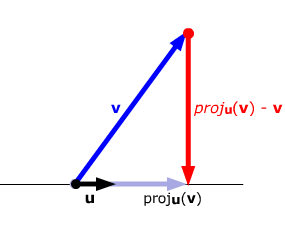
\includegraphics{projDeriv.png}
%![proyección ortogonal](projDeriv.png)

Si $\pb$ es la proyección de $\vb$ sobre $\langle \ub \rangle$, se cumple que $\pb-\vb$ es perpendicular a $\ub$. Es decir
$$
\langle \pb - \vb, \ub \rangle = 0.
$$

Aa la vez, $\pb = a \ub$, para un valor $a \in \R$ que podemos hallar resolviendo la ecuación
$$
0 = \langle \pb - \vb, \ub \rangle = \langle a\ub - \vb, \ub \rangle = a \langle \ub , \ub \rangle - \langle \vb, \ub \rangle.
$$

Obtenemos: $a = \frac{\langle \ub, \vb\rangle}{\langle \ub, \ub\rangle}$.

Es decir,
$$
\pb = \frac{\langle \ub, \vb \rangle}{\langle \ub, \ub \rangle} \ub.
$$

\begin{ejercicio}
Hallar la proyección del vector $(1,2)$ sobre la recta generada por el vector $(1,0)$ y la proyección de $(1,0)$ sobre la recta generada por $(1,2)$.

\begin{lstlisting}[language=R]
u = c(1,0)
v = c(1,2)
p = sum(u*v)/sum(u*u) * u
print(p)

q = sum(v*u)/sum(v*v) * v
print(q)
\end{lstlisting}
\end{ejercicio}

\subsection{Bases ortogonales - Proceso de Gram-Schmidt}

Dado un conjunto de vectores $\{\xb_1, \dots, \xb_s\}$ (linealmente independientes) el proceso de Gram-Schmidt permite obtener un nuevo conjunto ortogonal de vectores $\{\ub_1, \dots, \ub_s\}$ tal que $\langle \xb_1, \dots, \xb_t\rangle = \langle \ub_1, \dots, \ub_t\rangle$ para todo $1 \le t \le s$.

El proceso consiste en restarle a cada vector $\xb_i$ sus componentes en los vectores anteriores.

Construimos los vectores $\ub_i$ de la siguiente forma
\begin{itemize}
\item   $\ub_1 = \xb_1$
\item   $\ub_2 = \xb_2 - \frac{\langle \ub_1, \xb_2 \rangle}{\langle \ub_1, \ub_1 \rangle} \ub_1$
\item   $\ub_3 = \xb_3 - \frac{\langle \ub_1, \xb_3 \rangle}{\langle \ub_1, \ub_1\rangle} \ub_1 - \frac{\langle \ub_2, \xb_3 \rangle}{\langle \ub_2, \ub_2 \rangle} \ub_2$
\item   $\dots$
\item $\displaystyle{\ub_t = \xb_t - \sum_{i = 1}^{t-1} \frac{\langle \ub_i, \xb_t \rangle}{\langle \ub_i, \ub_i\rangle} \ub_i = \xb_t - \sum_{i = 1}^{t-1} \proj_{\ub_i}(\xb_t)}$, donde $\proj_{\ub}(\xb)$ es la proyección de $\xb$ sobre la recta generada por $\ub$ que definimos previamente.
\end{itemize}

En algunos casos, es conveniente utilizar vectores ortonormales (es decir ortogonales y de norma 1). En ese caso, podemos normalizar los vectores obtenidos mediante la fórmula
$$\wb_i = \frac{\ub_i}{\|\ub_i\|}, \quad 1 \le i \le t.$$

\begin{ejercicio}
Aplicar el proceso de Gram-Schmidt a los vectores $\xb_1 = (1, 0, 0)$, $\xb_2 = (2, 3, -1)$ y $\xb_3=(0, 7, -2)$.

\begin{lstlisting}[language=R]
x1 = c(1, 0, 0)
x2 = c(2, 3, -1)
x3 = c(0, 7, 2)

# Hacemos la cuenta para u2:
u1 = x1
u2 = x2 - sum(u1*x2)/sum(u1 * u1) * u1
print(u1)
print(u2)
print(u2 / sqrt(sum(u2^2)))

A = cbind(x1, x2, x3)
gS = gramSchmidt(A)
print(gS)
#gS$Q %*% t(gS$Q)
\end{lstlisting}
\end{ejercicio}


Dado un subespacio vectorial $V = \langle \vb_1, \dots, \vb_s \rangle \subset \R^n$, decimos que un conjunto de vectores $\{\wb_1, \dots, \wb_t\}$ es una base ortonormal de $V$ si

\begin{itemize}
\item $\|\wb_i\| = 1$ para todo $1 \le i \le t$.
\item $\langle \wb_i, \wb_j \rangle = 0$ para $i \neq j$.
\end{itemize}

Dada una base cualquiera $\B$ de un espacio vectorial, podemos obtener una base ortonormal aplicando el proceso de Gram-Schmidt.

\subsubsection{Proyección de un vector sobre un subespacio}

Ahora podemos extender la proyección de un vector sobre un subespacio cualquiera.

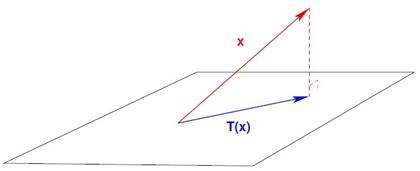
\includegraphics{proyeccionPlano.png}
%![](proyeccionPlano.png){width="220"}

Dado un subespacio vectorial $V \subset \R^n$ con base ortonormal $\B = \{\wb_1, \dots, \wb_s\}$ y un vector $\xb \in \R^n$, la proyección ortogonal de $\xb$ sobre $V$ se puede calcular por la fórmula

$$
\proj_V(\xb) = \sum_{i = 1}^{s} \proj_{\wb_i}(\xb)
$$

(comparar con la fórmula general del proceso de Gram-Schmidt).

\subsection{Matrices ortogonales}

Recordemos que una matriz $\Ab \in \mathbb{R}^{n \times n}$ es ortogonal si $\Ab \Ab^T = I_n$. Si $f_1, \dots, f_n$ son las filas de $\Ab$, $\Ab$ es ortogonal si
$$
\langle f_i , f_j\rangle =
\begin{cases}
1 & \text{ si } i = j \\
0 & \text{ si } i \ne j
\end{cases}.
$$
Es decir, todas las filas tienen norma-2 igual a 1 y son perpendiculares entre sí.

\begin{ejercicio}Verificar que la matriz
$$
\Ab = \begin{pmatrix}
1 & 0 & 0 \\ 0 & \cos \alpha & -\sin \alpha \\ 0 & \sin \alpha & \cos \alpha
\end{pmatrix}
$$
es una matriz ortogonal para cualquier valor de $\alpha$.
\end{ejercicio}

\begin{prop} Si $\Ab$ es una matriz ortonormal, la transformación lineal asociada conserva productos internos, y por lo tanto, preserva ángulos y distancias.

$$
\langle \Ab\ub, \Ab\vb \rangle = \langle \Ab^T \Ab \ub, \vb \rangle = \langle \ub, \vb \rangle
$$ Estas transformaciones se llaman isometrías o transformaciones rígidas del plano.
\end{prop}

\begin{ejercicio}
Interpretar geométricamente la transformación lineal asociada a la matriz del último ejercicio.

%\includegraphics{rotacionAlfa.gif}
%![rotación](rotacionAlfa.gif){width="200"}
\end{ejercicio}


** ESTO NO VA ACA PORQUE EN ESTA MATERIA TENEMOS OTRO CAPITULO PARA MINIMOS CUADRADOS **
\begin{aplicacion}[Aproximación por mínimos cuadrados]

Dados $n$ puntos en el plano, queremos calcular la recta que mejor aproxime esos puntos "en el sentido de mínimos cuadrados". Esto quiere decir, la recta tal que la suma de los errores cuadráticos que cometemos en las aproximaciones sean lo menor posibles.

Una forma de hacerlo es mediante proyecciones ortogonales.

\textbf{Ejemplo}

Dada la siguiente tabla de valores:

|     |     |     |     |     |
|-----|-----|-----|-----|-----|
| x   | 2   | 3   | 5   | 6   |
| y   | 5   | 7   | 10  | 11  |

queremos encontrar la recta $y = a+bx$ que mejor aproxima estos valores. Es decir, que los errores que cometemos $|y_i - (a+b x_i)|$ sean pequeños para los datos $(2, 5)$, $(3, 7)$, $(5, 10)$, $(6, 11)$.

\begin{lstlisting}[language=R]
x = c(2,3,5,6)
y = c(5,7,10,11)
plot(x, y, type = "p")
\end{lstlisting}

En el método de mínimos cuadrados, vamos a minimizar la suma de los errores cuadráticos:

$$
\sum_{i = 1}^4 (y_i - (a + bx_i))^2.
$$

Observemos que si pudieramos resolver exactamente el siguiente sistema de ecuaciones

$$
\left\{ {
\begin{alignedat}{5}
a&\;+\;&2b&\;=\;&5\\
a&\;+\;&3b&\;=\;&7 \\
a&\;+\;&5b&\;=\;&10\\
a&\;+\;&6b&\;=\;&11&,
\end{alignedat}}
\right.
$$entonces los errores serían todos $0$.

Sin embargo, en general un sistema con 4 ecuaciones y 2 incógnitas (¿quiénes son las incógnitas?) no tiene solución (verificarlo en este ejemplo). Por eso buscamos una solución aproximada. Para eso, escribimos el sistema en notación matricial:

$$\begin{pmatrix}1&2\\ 1 & 3 \\ 1 & 5 \\ 1 & 6 \end{pmatrix} \cdot \begin{pmatrix}a\\ b \end{pmatrix} = \begin{pmatrix}5\\ 7 \\10 \\ 11 \end{pmatrix}$$ Utilizando la teoría que vimos de espacios vectoriales, los vectores que obtenemos en el lado izquierdo de la ecuación tomando $a, b \in \R$ son vectores de la imagen de la matriz $\begin{pmatrix}1&2\\ 1 & 3 \\ 1 & 5 \\ 1 & 6 \end{pmatrix}$ y el sistema no tiene solución porque el vector $(5, 7, 10, 11)$ no pertenece a la imagen de la matriz.

La fórmula de suma de cuadrados que queremos minimizar: $$
\sum_{i = 1}^4 (y_i - (a + bx_i))^2.
$$coincide con la distancia del vector $y = (5, 7, 10, 11)$ a un punto de $\im(A)$.

Repasando todo, minimizar la suma de cuadrados equivale a buscar el punto de $\im(A)$ más cercano al punto $y = (5, 7, 10, 11)$ y esto lo hacemos proyectando $y$ sobre el subespacio vectorial $\im(A)$!

Para esto, ortoganlizamos primero la base de $\im(A)$. Tomamos $\B = \{x_1 = (1,1,1,1), x_2 = (2,3,5,6)\}$ y aplicamos Gram-Schmidt.

\begin{itemize}
\item   $u_1 = x_1 = (1,1,1,1)$
\item $u_2 = x_2 - \frac{\langle u_1, x_2 \rangle}{\langle u_1, u_1\rangle} u_1 = (2,3,5,6) - \frac{\langle (1,1,1,1), (2,3,5,6) \rangle}{\langle (1,1,1,1), (1,1,1,1)\rangle} (1,1,1,1) = (2,3,5,6) - 4 (1,1,1,1) = (-2, -1, 1, 2)$
\end{itemize}

Obtenemos la base ortogonal $\mathcal{O} = \{u_1 = (1,1,1,1), u_2 = (-2, -1, 1, 2)\}$.

Finalmente calculamos la proyección: $$
\proj_{\im(A)}(y) = \frac{\langle u_1, y\rangle}{\langle u_1, u_1\rangle} u_1 + \frac{\langle u_2, y\rangle}{\langle u_2, u_2\rangle} u_2 = (?,?,?,?).
$$

\begin{lstlisting}[language=R]
u1 = c(1,1,1,1)
u2 = c(-2,-1,1,2)
y = c(5,7,10,11)
# El comando drop convierte una matrix de 1x1 a escalar
p = drop((t(u1) %*% y) / (t(u1) %*% u1)) * u1 + drop((t(u2) %*% y) / (t(u2) %*% u2)) * u2
print(p)
\end{lstlisting}

$$
\proj_{\im(A)}(y) =  (5.25, 6.75, 9.75, 11.25).
$$

El último paso es encontrar $(a,b)$. Para esto, escribimos a $y$ en la base $\B$, resolviendo el sistema

$$
a(1,1,1,1) + b (2,3,5,6) = (5.25, 6.75, 9.75, 11.25)
$$

\begin{lstlisting}[language=R]
# Usamos solo las primeras dos ecuaciones
A2 = matrix(c(1,1,2,3), nrow = 2)
print(A2)
y2 = c(5.25, 6.75)
c = solve(A2, y2)
print(c)
\end{lstlisting}


\begin{lstlisting}[language=R]
# Verificamos
A = matrix(c(1,1,1,1,2,3,5,6), nrow = 4)
y = c(5.25, 6.75, 9.75, 11.25)
A %*% c
\end{lstlisting}


Obtenemos $(a, b) = (2.25 , 1.5)$.

\textbf{Conclusión:}

La recta que mejor aproxima los datos en el sentido de mínimos cuadrados es $y = 2.25 + 1.5 x$.

Graficamos todos los datos para verificar que obtuvimos una buena aproximación.

\begin{lstlisting}[language=R]
x = c(2,3,5,6)
y = c(5,7,10,11)
plot(x, y, type = "p")

x_plot = 0:6
y_plot = 1.5*x_plot +2.25
lines(x_plot, y_plot, col = "green")
\end{lstlisting}


\textbf{Otra forma más práctica}

Buscar $(a,b)$ para los cuales el vector $p = a x_1 + b x_2 \perp y-p$.

\end{aplicacion}


\subsection{Normas de matrices}

Dada una matriz $\Ab \in \R^{n \times n}$, y una norma vectorial $\|\cdot\|_p$ en $\R^n$, podemos definir una norma asociada $\|\Ab\|_p$ por

$$
\|\Ab\|_p = \max_{\xb \in \R^n - \{0\}} \frac{\|\Ab\xb\|_p}{\|x\|_p} = \max_{\xb \in \R^n, \|\xb\|_p = 1} \|\Ab\xb\|_p.
$$

Es decir, la norma de una matriz mide en qué proporción puede aumentar como máximo la norma de un vector $\xb$ al multiplicarlo por $\Ab$.

\begin{prop}\leavevmode
\begin{itemize}
\item Si $\Ab$ es simétrica, $\|\Ab\|_2 = \rho(\Ab) = |\lambda_{\max}|$.
\item Para $\Ab$ arbitraria, $\|\Ab\|_2 = \sigma_{\max}$ , el mayor ¡valor singular!
\item En general, para $\Ab$ arbitraria se tiene $\rho(\Ab) = \inf_{\|\cdot\|} \|\Ab\|$. En particular, $\rho(\Ab) \le \|\Ab\|$ para cualquier norma matricial.
\end{itemize}
\end{prop}
